\documentclass[letterpaper, 12pt]{report}

% insert any packages, environments, counters, etc here
\usepackage{graphicx}
\usepackage{hyperref}


\begin{document}
%insert document contents here

The following practical design process is recommended: 

\begin{itemize}
\item Determine your goals : what error metric to use, and the target value for the metric.
\item Establish a working end to end pipeline as soon as possible, including the estimation of the appropriate performance metrics 
\item Instrument the system to determine bottlenecks in performance. 
\item Repeatedly make incremental changes such as gathering new data, adjusting hyperparameters, or changing algorithms based on specific findings from our instrumentation.
\end{itemize}
 
\section{11.1 | Performance Metrics}

Sometimes it is more costly to make one mistake than another. As an example, we may want to focus on measuring \textbf{precision} and \textbf{recall}. 

Precision is the fraction of detectings that were reported by the model that were correct (true positives), while recall is the fraction of true events that were detected (true positives / true positives + true negatives). 

If we wish to summarize the performance of a classifier with a single number rather than a score, we can convert precision and recall into an \textbf{F-score} given by 

\begin{center}
  $F = \frac{2pr}{p + r}$
\end{center}

Another option is to report the total area lying beneath the PR curve. 

In some applications, we can control whether a machine learning model makes a decision or not. A natural performance metric to use for this situation is called \textbf{coverage}. Coverage is the fraction of examples for which a machine learning system is able to produce a response. It is possible to trade coverage for accuracy. 

What is important is to determine which performance metric to improve ahead of time, then concentrate on improving this metric. Without clearly defined goals, it can be difficult to tell whether changes to a machine learning system make progress or not. 

\section{11.2 | Default Baseline Methods}

Depending on the complexity of the problem, its good to start with a simpler (non-deep) model. 

First choose the general category of model based on the structure of our data. 

\begin{itemize}
\item If we wish to wish to use fixed size vectors as input, use a feedforward network with fully connected layers.
\item If the input has a known topological structure, use a convolutional network. In this cases, begin with a piecewise linear unit (ReLUs or their generalizations like Leaky ReLUs, PreLus, or Maxout). 
\item If the input is a sequence, use a gated recurrent net (LSTM or GRU)
\item A reasonable optimization algorithm is SGD with momentum and a decaying learning rate or Adam 
\item Batch norm can have a dramatic effect on performance, especially with convnets and networks with sigmoidal nonlinearities. 
\item Unless our training set contains tens of millions of data points, we should use regularization from the start. 
\item Early stopping, and dropout OR batch normalization should be used to reduce generalization error. 
\item Decide whether to use unsupervised learning. Some domains like NLP benefit heavily from it, whereas convnets benefit less unless used in a semi-supervised manner.
\end{itemize}

\href{https://arxiv.org/pdf/1507.02672.pdf}{Semi-Supervised Learning with Ladder Networks | Rasmus et al 2015}

\begin{quote}
  \textbf{Abstract: } We combine supervised learning with unsupervised
  learning in deep neural networks. The proposed model is trained to
  simultaneously minimize the sum of supervised and unsupervised cost
  functions by backpropagation, avoiding the need for layer-wise
  pre-training. Our work builds on the Ladder network proposed by
  Valpola (2015), which we extend by combining the model with
  supervision. We show that the resulting model reaches
  state-of-the-art performance in semi-supervised MNIST and CIFAR-10
  classification, in addition to permutationinvariant MNIST
  classification with all labels.
\end{quote}

Which provides the following directions: 

\textbf{General Steps for Implementing the Ladder Network} 
Consider training a classifier or a mapping from input x to output y with
targets t, from a training set of pairs ${x(n), t(n) | 1 \leq n \leq
N}$. Semi-supervised learning (Chapelle et al., 2006) studies how
auxiliary unlabeled data ${x(n) | N + 1 \leq n \leq M}$ can help in training a
classifier. It is often the case that labeled data are scarce whereas
unlabeled data are plentiful, that is $N <<  M$.  The Ladder network can
improve results even without auxiliary unlabeled data but the original
motivation was to make it possible to take well-performing feedforward
classifiers and augment them with an auxiliary decoder as follows:

1. Train any standard feedforward neural network. The network type is
not limited to standard MLPs, but the approach can be applied, for
example, to convolutional or recurrent networks. This will be the
encoder part of the Ladder network.  

2. For each layer, analyze the conditional distribution of
representations given the layer above, $p(z(l) | z (l+1))$. The
observed distributions could resemble for example Gaussian
distributions where the mean and variance depend on the values $z^{(l+1)}$, bimodal distributions where the relative probability masses of
the modes depend on the values $z^{(l+1)}$, and so on.

3. Define a function $z^{(l)} = g(z^{~(l)}, \hat{z}^{(l+1)})$ which can
approximate the optimal denoising function for the family of observed
distributions. The function g is therefore expected to form a
reconstruction $\hat{z}^{(l)}$ that resembles the clean $z^{(l)}$ given the
corrupted $z^{~(l)}$ and the higher-level reconstruction $\hat{z}^{(l+1)}$ .

4. Train the whole network in a fully-labeled or semi-supervised
setting using standard optimization techniques such as stochastic
gradient descent.

\href{https://arxiv.org/pdf/1406.5298.pdf}{Semi-supervised Learning with Deep Generative Models | Kingma et al 2014}

\begin{quote}
  \textbf{Abstract: } The ever-increasing size of modern data sets
  combined with the difficulty of obtaining label information has made
  semi-supervised learning one of the problems of significant
  practical importance in modern data analysis. We revisit the
  approach to semi-supervised learning with generative models and
  develop new models that allow for effective generalisation from
  small labelled data sets to large unlabelled ones. Generative
  approaches have thus far been either inflexible, inefficient or
  non-scalable. We show that deep generative models and approximate
  Bayesian inference exploiting recent advances in variational methods
  can be used to provide significant improvements, making generative
  approaches highly competitive for semi-supervised learning.
\end{quote}

Only use unsupervised learning in the first go if the problem is a context in which unsupervised learning is known to be important. We can always add unsupervised learning later if the initial baseline overfits or underfits. 

\section{11.3 | Determining Whether to Gather More Data }

If the test set performance is much worse than the training set performance, then gathering data is one of the most effective solutions. 

\section{11.4 | Selecting Hyperparameters}

There are two approaches to selecting hyperparameters: 

\begin{itemize}
\item choosing manually 
\item choosing automatically
\end{itemize}

\subsection{11.4.1 | Manual Hyperparameter Tuning}

The goal of manual hyperparameter search is usually to find the lowest generalization error subject to some runtime and memory budget. The primary goal is to adjust the effective capacity of the model to match the complexity of the task. 

Effective capacity is constrained by 3 factors: 

\begin{itemize}
\item the representational capacity of the model 
\item the ability of the learning algorithm to successfully minimize the cost function used to train the model 
\item the degree to which the cost function and training procedure regularize the model
\end{itemize}

A model with more layers and hidden units per layer has higher representational capacity - it is capable of representing more complicated functions. 

The learning rate is perhaps the most important hyperparameter. If we have time to tune only one parameter, tune the learning rate. The effective capacity of the model is highest when the learning rate is correct for the optimization problem, not when the learning rate is especially large or small. 

Tuning the parameters other than the learning rate requires monitoring both training and test error to diagnose whether the model is overfitting or underfitting, and then adjusting its capacity appropriately. If the error on the training set is higher than the target error rate, we have no choice but to increase capacity. If we are not using regularization and are confident that our optimization algorithm is working correctly, then we must add more layers or add more hidden units. 

If the error on the test set is higher than our target error rate, we can usually fix this by changing regularization hyperparameters to reduce effective model capacity, such as adding dropout or weight decay. Usually the best performance comes from a large model that is regularized well. 

\begin{figure}[h]
  \centering
  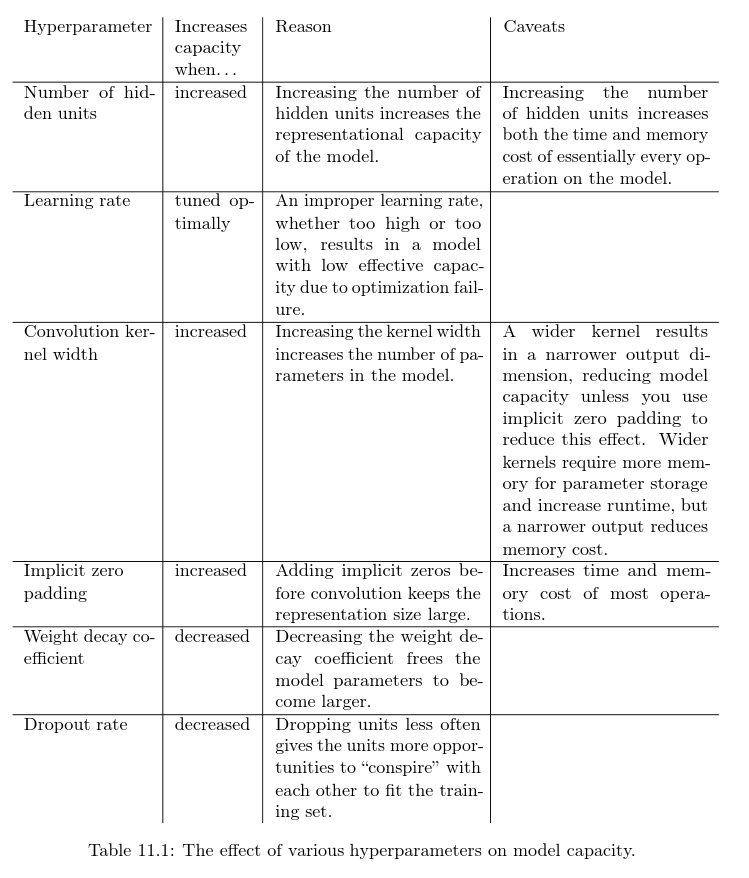
\includegraphics[width=0.7\textwidth]{hyperparam_model_capacity.png}
\end{figure}

\subsection{11.4.2 | Automatic  Hyperparameter Optimization Algorithms}

\textbf{Grid Search}

When there are three or fewer parameters, it is common practice to perform grid search. Typically a grid search involves picking values approximately on a logarithmic scale. Grid search usually performs best when it is performed repeatedly. For example, if we were seeking an optimal hyperparameter $\alpha$ using the values $\{-1, 0, 1\}$ and the best value we found is 1, then we may shift the space to $\{2, 3, 4\}$ or close in with $\{0.8, 0.9, 1,  1.1, 1.2\}$. The downside is the time complexity, $O(n^m)$, but this can be ran in parallel. 

\textbf{Random Search}

First we define a marginal distribution for each hyperparameter, for example a Bernoulli or Multinoulli for binary or discrete hyperparameters, or a uniform on a log scale for positive real valued hyperparameters. Unlike in grid search, we should not discretize or bin the values of the hyperparameters, so that we can explore a larger set of values and avoid additional computational cost. 

\textbf{Model-Based Hyperparameter Optimization}

We can cast the search for good hyperparameters as an optimization problem in which the decision variables are the hyperparameters, and the cost to be optimized is the validation set error that results from training using these hyperparameters. 

In some cases we can simply use gradient descent. In cases where this doesn't work, we can build a model of the validation set error and propose new hyperparameter guesses by performing optimization within this model. 

Most model based algorithms for hyperparameter search use a Bayesian regression model to estimate both the expected value of the validation set error for each hyperparameter and the uncertainty around this expectation. Optimization thus involves a tradeoff between exploration (proposing hyperparameters for which there is high uncertainty) and exploitation (hyperparameters similar to what it knows works so far). 

\section{11.5 | Debugging Strategies}

There are two main difficulties with debugging networks:

\begin{enumerate}
\item When a machine learning system performs poorly, it is difficult to tell whether the poor performance is intrinsic to the algorithm or whether there is a bug in the implementation of the algorithm 
\item Each model tends to have multiple parts that are adaptive. If one part is broken, the other parts can adapt and still achieve roughly acceptable performance, masking the inefficiency. 
\end{enumerate}

Most debugging centers around one or both of these difficulties.

Some important bugging tests: 

\begin{itemize}
\item visualize the model in action. Look at examples 
\item visualize the worst mistakes 
\item reason about software usin training and test error
\item fit a tiny dataset 
\item monitor histograms of activations and gradients 
\end{itemize}

\end{document}